\section{Program}

\subsection{Architektura programu}

%%%%%%%%%%%%%%%%%%%%%%%%%%%%%%% OGRANICZENIA %%%%%%%%%%%%%%%%%%%%%%%%%%%%%%

\textbf{Ograniczenia} wprowadzone do programu zastosowano w~celu zmniejszenia stopnia złożoności projektów i~uproszczenia użytkownikowi tworzenia projektów.

Podstawowymi ograniczeniami są: minimalne wymiary obszaru wynoszące $8 \times 8$ pikseli oraz maksymalnie osiem obszarów w~projekcie. Rozmiar najmniejszego znaku wyświetlanego przez tablicę wynosi $8 \times 8$, z~czego wynika ograniczenie dotyczące minimalnych wymiarów obszaru. W~każdym obszarze tekstowym zabronione jest umieszczanie tekstu większego niż wysokość obszaru.

Ponadto dwa obszary nie mogą nakładać się na siebie, jeśli nie są w~relacji całkowitego zawierania się w~sobie. Restrykcja została wprowadzona aby uniknąć sytuacji gdy dwa poruszające się teksty mieszałyby się ze sobą, co byłoby nieczytelne i~niefunkcjonalne. Obszar może zostać umieszczony albo całkowicie wewnątrz innego obszaru, albo całkowicie na zewnątrz.

Następne ograniczenia wiążą się z~zagnieżdżeniem obszarów. Obszar będący wewnętrznym obszarem musi zawierać tekst, natomiast obszar zewnętrzny musi zawierać tylko i~wyłącznie grafikę. Obszar graficzny wewnątrz obszaru graficznego byłby niepotrzebną strukturą, ponieważ użytkownik mając jeden obszar graficzny ma pełną dowolność w~wypełnianiu go. Dodatkowo jeśli jakiś obszar posiada już wewnątrz siebie inny obszar, nie może mieścić w~sobie już kolejnego obszaru. Relacje zagnieżdżenia obszarów zostały ograniczone do 1 : 1 (na jeden korzeń przypada tylko jeden liść i~na odwrót).

Istnieją również ograniczenia dotyczące obramowań obszarów. Żadne obramowania obszarów, niezależnie od relacji między nimi (wewnętrzna/zewnętrzna), nie mogą nakładać się na siebie. Dzięki temu nie ma możliwości pełnego powielenia obszaru i~niemożliwa jest sytuacja, gdy obydwa obszary zajmują te same komórki w~tablicy i~nie można wybrać kursorem myszki obszaru ,,pod spodem'' chcąc dodać mu treść.

Wszystkie z~tych ograniczeń zostały uwzględnione i~zaimplementowane w~aplikacji. Natychmiast podczas naruszania ograniczenia program powiadamia użytkownika lub uniemożliwia wykonanie akcji --- np. nie jest możliwe skrzyżowanie lub nałożenie się na siebie dwóch obszarów. Rysowany obszar zatrzyma się na granicy innego obszaru. Ograniczenia dotyczące projektowania obszarów tekstowych zostaną omówione w~dalszej części pracy.

%%%%%%%%%%%%%%%%%%%%%%%%%%%%% EFEKTY ANIMACJI %%%%%%%%%%%%%%%%%%%%%%%%%%%%%%%%%

\textbf{Zaimplementowane efekty animacji} podzielone są na efekty graficzne i~tekstowe. W~trybie edycji graficznej jedynym dostępnym efektem jest negatyw. Jego działanie polega na odwróceniu wszystkich wartości w~tabeli obszaru, a~więc zamianie wszystkich zer na jedynki i~na odwrót.

\begin{figure}[htb]
	\begin{center}
		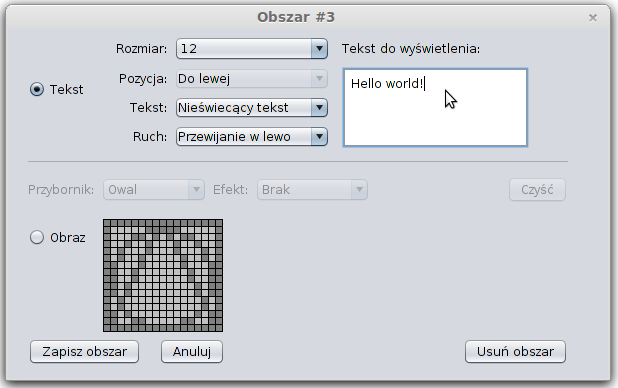
\includegraphics[width=0.8\textwidth]{figures/areaText.png}
	\end{center}
	\caption{Edycja obszaru w trybie tekstowym.}
\end{figure}

W trybie edycji tekstowej zaimplementowano więcej efektów. Dzielą się na cztery kategorie: \textit{rozmiar}, \textit{pozycja}, \textit{wyświetlanie tekstu} oraz \textit{ruch}. Poniżej omówiono krótko każdą z~kategorii z~wypisanymi opcjami.

Rozmiar:

\begin{itemize}
	\item \textit{8} --- rozmiar zawsze dostępny z~uwagi na minimalną wysokość obszaru równą 8,
	\item \textit{12} --- rozmiar dostępny dla wysokości obszaru większej lub równej 12,
	\item \textit{16} --- rozmiar dostępny dla wysokości obszaru równej 16.
\end{itemize}

Pozycja:

\begin{itemize}
	\item \textit{Do lewej} --- wyrównanie tekstu do lewej,
	\item \textit{Wyśrodkowane} --- wyśrodkowanie tekstu,
	\item \textit{Do prawej} --- wyrównanie tekstu do prawej.
\end{itemize}

Wyświetlanie tekstu:

\begin{itemize}
	\item \textit{Świecący tekst} --- wprowadzony napis będzie pokazywany przez zapalone diody. Widoczny tylko na tle składającym się ze zgaszonych diod.
	\item \textit{Nieświecący tekst} --- wprowadzony napis będzie pokazywany przez zgaszone diody. Widoczny tylko na tle składającym się z~zapalonych diod.
	\item \textit{Negatyw tła} --- wprowadzony napis będzie pokazywany przez zgaszone diody na zapalonym tle oraz zapalone diody na zgaszonym tle. Widoczny na każdym tle.
\end{itemize}

Ruch:

\begin{itemize}
	\item \textit{Brak} -- brak efektu, tekst wypisywany według wskazanego wyrównania w~\textit{Pozycji},
	\item \textit{Odbijanie w~poziomie} -- tekst odbijany od bocznych krawędzi obszaru,
	\item \textit{Odbijanie w~pionie} -- tekst odbijany od górnej i~dolnej krawędzi obszaru,
	\item \textit{Przewijanie w~lewo} -- tekst przewijany od prawej krawędzi obszaru do lewej,
	\item \textit{Przewijanie w~górę} -- tekst przewijany z~pod dolnej krawędzi obszaru nad górną,
	\item \textit{Przewijanie w~dół} -- tekst przewijany z~nad górnej krawędzi obszaru pod dolną.
\end{itemize}

Aby zaciemnić pojedyncze elementy kontrolki \texttt{JComboBox} należało zaimplementować własną klasę \texttt{MyComboBox} \cite{jcombobox}. Z~uwagi na fakt, iż nie wszystkie pary efektów można stosować w~tym samym czasie zaimplementowano wyłączanie całych kontrolek lub niektórych ich elementów w~zależności od ustawienia pozostałych efektów. Poniżej wypisano wszystkie zaimplementowane zależności.

\begin{itemize}
	\item Jeśli długość tekstu wpisanego przez użytkownika jest większa niż długość obszaru, cała kontrolka \textit{Pozycja} oraz wszystkie elementy kategorii \textit{Ruch} za wyjątkiem \textit{Przewijania w~lewo} zostają zaciemnione. Powodem jest fakt, iż tekst musi być wyświetlony w~całości, a~więc poza przesunięciem tekstu w~lewo nie ma sposobu, aby w~pełni go zaprezentować.
	\item Jeśli \textit{Ruch} zostanie ustawiony na \textit{Odbijanie w~poziomie} lub \textit{Przewijanie w~lewo}, zaciemniona zostaje cała kontrolka \textit{Pozycja}. Gdy tekst rusza się w~poziomie, nie ma potrzeby wyrównywać go w~tej płaszczyźnie.
	\item Jeśli wysokość obszaru jest równa opcji zaznaczonej w~efekcie \textit{Rozmiar}, zaciemniony zostaje element \textit{Odbijanie w~pionie} w~kontrolce \textit{Ruch}. Podobnie dzieje się z~\textit{Odbijaniem w~poziomie}, gdy szerokość obszaru i~długość tekstu są równe.
\end{itemize}

%%%%TUTAJ GDZIEŚ RYSUNEK


%%%%%%%%%%%%%%%%%%%%%%%%%%%% EDYTOR %%%%%%%%%%%%%%%%%%%%%%%%%%%%%%

\textbf{W edytorze}, główną strukturą, na której oparty jest interfejs użytkownika, jest tablica zmiennych typu \texttt{byte} o~rozmiarach $128 \times 16$ inicjowana i~wypełniana zerami po uruchomieniu programu. Jej stan jest bezpośrednio pokazywany na ekranie podczas działania programu --- tabela jest przerysowywana podczas każdego ruchu kursora myszki, lub wywoływana jawnie podczas niektórych zdarzeń np. utworzenie nowego obszaru. W~zależności od zawartości komórki w~tabeli rysowany jest kwadrat (piksel) o~różnym kolorze. Czarnym kolorem oznaczone są granice obszaru --- jest on pustym wewnątrz prostokątem. Kolor biały jest zarówno wewnątrz, jak i~na zewnątrz obszaru. Wyjątkiem jest moment, w~którym kursor myszki znajdzie się nad obszarem --- wtedy wypełniany jest on szarym kolorem stwarzając efekt podświetlenia.

\begin{figure}[htb]
	\begin{center}
		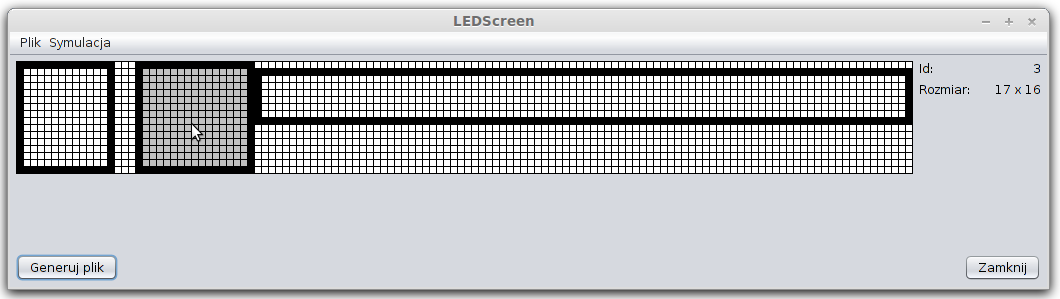
\includegraphics[width=\textwidth]{figures/gui2.png}
	\end{center}
	\caption{Główne okno programu z podświetlonym obszarem.}
\end{figure}

Zawartość komórki została podzielona na część dziesiętną i~część jedności, pełniące odmienne funkcje. Część dziesiętna liczby wewnątrz komórki przeznaczona jest na identyfikator obszaru. Indeksowanie obszarów rozpoczyna się od identyfikatora 1. Gdy w~komórce w~części dziesiętnej pozostaje 0 oznacza to, że dany piksel nie należy do żadnego z~obszarów i~nie będzie używany podczas animacji. Część jedności liczby w~komórce tabeli wynosi 1 albo 2. Jeśli kursor myszki znajdzie się nad miejscem odpowiadającym komórce z~częścią jedności równą 1, oznacza to, że znalazł się na obramowaniu obszaru, a~jeśli część jedności wartości komórki odwiedzonej przez kursor wynosi 2, na jego wypełnieniu. Przykład: jeśli kursor myszki znajdzie się nad komórką 52 oznacza to, że znalazł się nad wypełnieniem obszaru o~identyfikatorze 5. 

Część jedności w~tablicy może mieć jeszcze jedną, chwilową wartość równą 3. Taka wartość jest przyjmowana gdy kursor myszki będzie nad danym obszarem (nad komórką z~częścią dziesiętną równą identyfikatorowi obszaru) i~spowoduje podświetlenie całego obszaru. Gdy kursor napotka komórkę z~wartością 0 lub z~innym identyfikatorem (częścią dziesiętną), wartość części jedności z~poprzednio podświetlonego obszaru powróci do wartości 2. Oto przykład dla poprzedniej sytuacji z~komórką o~wartości 52: tak długo, jak kursor będzie nad obszarem o~identyfikatorze 5 wszystkie wartości 52 zostaną zamienione na 53, dopiero w~momencie opuszczenia przez kursor obszaru o~identyfikatorze 5 komórki jego wypełnienia wrócą do wartości 52.

Klasa \texttt{Area} jest klasą przechowującą wszystkie parametry obszaru takie jak współrzędne początkowego i~końcowego narożnika, szerokość, wysokość oraz ustawienia dotyczące efektów tekstowych i~graficznych. W~klasie obszaru znajduje się również metoda \texttt{String getTTextChars()}, która zamienia ciąg znaków wprowadzony przez użytkownika na ciąg zrozumiały dla mikroprocesora zawierający znaki specjalne (np. cyfra dziesiętna godziny albo dnia miesiąca). Każdy obiekt klasy \texttt{Area} ma pole \texttt{String type}, które przyjmuje wartość ,,picture'' lub ,,text'', odpowiednio dla obszaru graficznego i~tekstowego, w~zależności od typu, który użytkownik chce mu nadać. Dodatkowo wszystkie obiekty obszarów mają dwa pola typu \texttt{Area} o~nazwach \texttt{parent} i~\texttt{child}. Zależnie od usytuowania obszarów względem siebie zapisują w~nich rodzica (jeśli są w~nim zagnieżdżone), potomka (jeśli jest zagnieżdżony w~nich), lub żadnego z~nich (wtedy obydwa pola ustawiane są na \texttt{null}).

Wszystkie obszary narysowane lub wczytane są dodawane do globalnej listy o~nazwie \texttt{areas}. Gdy obszar jest usuwany, pola \texttt{parent} i~\texttt{child} powiązanych z~usuwanym obiektem obszarów są odpowiednio ustawiane na wartość \texttt{null}, w~zależności od relacji. Po usunięciu obszaru aktualizowane są identyfikatory wszystkich obszarów: puste miejsce na liście zastępowane jest przez następnik usuniętego elementu i~podobnie aktualizowany jest identyfikator. Następuje przesunięcie identyfikatorów następników usuniętego obiektu o~jeden, a~główna tablica (części dziesiętne komórek przechowujące identyfikator obszaru) uaktualniana. Aby podczas usuwania umożliwić powrót do stanu sprzed istnienia usuwanego obszaru każdy obiekt klasy \texttt{Area} posiada pole \texttt{background}, do którego już podczas inicjacji obiektu zapisywana jest wartość komórek głównej tablicy sprzed powstania tego obszaru. Dzięki temu obszar zapamiętuje, co było ,,pod'' nim i~jaką wartość musi ustawić w~głównej tablicy podczas usuwania. Zmienna background jest również uaktualniana podczas usuwania obszarów, gdy uaktualniane są identyfikatory.

W graficznym trybie edycji obszaru wyświetlane są komórki ,,właściwe'' obszaru, czyli tabela z~wartościami zero lub jeden. Zero oznacza, że dioda na tablicy odpowiadająca temu pikselowi będzie zgaszona, jeden oznacza zapaloną diodę. Do dyspozycji użytkownika zaimplementowano przybornik składający się ze zwykłego ołówka, linii prostej, trójkąta, prostokąta oraz owalu. Ołówek zamienia wartości komórek w~tablicy obszaru bezpośrednio, z~zera na jeden w~miejscu użycia, natomiast wszystkie figury w~momencie trzymania przycisku myszy przetrzymywane są w~nowej tymczasowej tablicy \texttt{temp} o~rozmiarach identycznych z~rozmiarami edytowanego obszaru. W~momencie puszczenia przycisku myszy tablica \texttt{temp} dodawana jest do tablicy obszaru operacją bitową OR na odpowiadających sobie komórkach.

Do zaimplementowania rysowania linii, a~przy jej pomocy trójkąta użyto algorytmu Bresenhama \cite{bresenham}. Otrzymywanie owalnego kształtu na powierzchni obszaru zostało zaimplementowane według algorytmu z~tego samego źródła \cite{ovals}. Wszystkie algorytmy graficzne zostały odpowiednio dostosowane do interfejsu np. owal nie jest rysowany od środka do obrzeży (tak jak w~źródle), lecz od lewego-górnego narożnika do prawego-dolnego.

W tekstowym trybie edycji użytkownik ma większe możliwości konfiguracyjne. Wpisany tekst do pola tekstowego jest na bieżąco ,,sprawdzany'' pod względem długości tekstu w~pikselach i~porównywany z~długością obszaru. Jeśli długość tekstu przekroczy długość obszaru, zaciemniane są te opcje, które nie mogą zostać zrealizowane przy dłuższym tekście. Reguła sprawdzania długości tekstu obejmuje również znaki specjalne --- ciąg znaków \texttt{$\backslash$g} nie jest odczytywany jako dwa znaki, lecz jako jeden.

%%%%%%%%%%%%%%%%%%%% GENERATOR PLIKU %%%%%%%%%%%%%%%%%%%%%%%

\textbf{Generator pliku animacji} o~rozszerzeniu \texttt{.m2f} uruchamiany jest po użyciu przycisku \textit{Generuj} w~lewym dolnym narożniku głównego okna programu. Za pomocą generatora jest również tworzony tymczasowy plik po wybraniu opcji \textit{Symuluj aktualny projekt} w~menu \textit{Symulacja} i~jego tworzenie przebiega w~identyczny sposób. Jedyna różnica to natychmiastowe usuwanie pliku tymczasowego po symulacji.

Działanie generatora plików jest wieloetapowe. Podczas inicjacji instancji generatora rozdzielane są wszystkie obszary dostępne w~projekcie na obszary tekstowe i~graficzne. Przydzielone są one do list przechowujących obiekty typu \texttt{Area} o~nazwach \texttt{backgroundAreas} oraz \texttt{textAreas} odpowiednio dla obszarów graficznych i~tekstowych. Dodatkowo inicjowana jest tablica z~identyfikatorami znaków potrzebnymi do ich wyświetlania. Jest to tablica o~rozmiarze 127 inicjowana tak, aby indeks tablicy odpowiadał wartości komórki o~tym indeksie. Taką strukturę zaimplementowano jako pulę identyfikatorów dla znaków pokazywanych na ekranie. Każdemu obszarowi przydzielana jest taka liczba identyfikatorów, ile jest w~stanie wyświetlić znaków w~jednym momencie. Takie postępowanie zapobiega mieszaniu się znaków ze sobą i~wzajemnego ich nadpisywania.

Podczas postępu w~wykonywaniu kodu generatora komendy dla mikroprocesora dodawane są do listy bajtów. Kończąc działanie program zapisze te bajty do pliku generując wynikowy plik animacji \texttt{.m2f}. Pseudokod obrazujący działanie generatora po zainicjowaniu tablicy z~identyfikatorami i~rozdzielonymi listami obszarów przedstawiony został poniżej:
\newpage
\begin{verbatim}
    dodajKomendySterujące();
    wczytajTło();

    if (obszaryTekstowe.ilość > 0) {
        generujKlatki();
        zapiszKlatkiDoTablicyBajtów(int : długośćNajdłuższejAnimacji);
    }

    zapiszTablicęBajtówDoPliku();
\end{verbatim}

Pierwszym etapem po inicjalizacji struktur jest wprowadzenie komend sterujących oraz tła: następne 256 bajtów jest wczytywane do głównej listy bajtów i~interpretowane jako tło animacji. Jeśli nie został utworzony obszar graficzny, wszystkie wartości będą miały wartość zero.

Najważniejszym etapem generacji pliku jest tworzenie ciągu klatek dla każdego z~obszarów. Po przejściu do następnej klatki znaki zmienią swoje położenie (o~ile w~kontrolce \textit{Ruch} nie zaznaczono elementu \textit{Brak}). W~obszarze zaimplementowano listę przechowującą klatki tego obszaru. Generacja pliku przebiega w~taki sposób, aby najpierw wygenerować całą listę klatek dla każdego obszaru tekstowego, a~następnie w~pętli je dodawać --- najpierw wpisywana jest pierwsza klatka każdego obszaru, potem druga, itd. Jeśli animacja jest tworzona dla więcej niż jednego obszaru, wyznaczana jest obszar z~najdłuższą animacją, a~pozostałe powtarzają swoje animacje aż do skończenia pokazu przez ten obszar.

Poniższy pseudokod prezentuje zapisywanie wygenerowanych intrukcji wewnątrz klatek do wynikowego pliku animacji \texttt{.m2f} (w~psuedokodzie pominięto sprawdzanie zakresów kolekcji):

\begin{verbatim}
    for (i : 0 .. <liczba_klatek_w_najdłuższej_animacji>)
        for (każdy obiekt area z listy obszarów)
            area.zbiorKlatek[i].getWszystkieInstrukcjeWKlatce();
\end{verbatim}

Klatka jest obiektem klasy o~nazwie \texttt{Frame} i~zawiera listę przechowującą instrukcje podane mikroprocesorowi podczas jednego odświeżenia aktualnych parametrów znaków. Instrukcja to obiekt klasy o~nazwie \texttt{Instruction} zawierająca trzy zmienne publiczne: \texttt{command}, \texttt{argument}, \texttt{value}, która służy do przechowywania podanych rozkazów. Taka implementacja pozwala na łatwy dostęp do instrukcji podanych w~konkretnej klatce. Jest możliwe również powielanie wybranych klatek, co znacząco ułatwia zapętlanie animacji poszczególnych obszarów aż do zakończenia najdłuższej animacji.

Na początku funkcji \texttt{generujKlatki()} wczytywane są znaki wprowadzone do tekstu obszaru i~zamieniane na obiekty typu \texttt{ScreenChar}, który zawiera wszystkie parametry znaku potrzebne mikrokontrolerowi, aby prawidłowo go wyświetlić, np. współrzędna pozioma i~pionowa narożnika początkowego, rozmiar, znak, identyfikator. Każdy znak zostaje sprawdzony, czy znajduje się na ekranie na podstawie wcześniej wymienionych parametrów. Jeśli tak, do listy instrukcji dodawane są instrukcje inicjalizujące znak na ekranie. Jeśli nie, znak jest pomijany (przypadek przewijania tekstu w~lewo) i~nie jest inicjalizowany w~tej chwili. W~zależności od ustawionego ruchu 
odpowiednia współrzędna wszystkich znaków w~obszarze jest zmniejszana bądź zwiększana np. przy zaznaczonej opcji ruchu \textit{Przesuwanie do góry} parametr współrzędnej pionowej znaku jest zmniejszany o~jeden (z~uwagi na fakt, iż początek układu współrzędnych znajduje się w~lewym-górnym narożniku). Dodatkowo jeśli znak znajduje się w~okolicy krawędzi obszaru dodawane są odcięcia, aby żaden znak nie wykraczał poza granice wyznaczane przez obszar. 

W przypadku przewijania tekstu w~lewo, gdzie szybko mogą skończyć się dostępne identyfikatory zastosowano ,,oddawanie'' identyfikatorów dla tych znaków, które już zostały wyświetlone i~znalazły się po drugiej stronie obszaru. ,,Oddają'' wtedy swój identyfikator (wartość ich identyfikatora przywracana jest do tabeli identyfikatorów inicjowanej na początku), dzięki czemu długość tekstu możliwa do wyświetlenia jest bardzo duża (nie ogranicza się do 127 identyfikatorów). Na ekranie mogą być maksymalnie 64 znaki w~tej samej chwili. Dzięki odzyskiwaniu identyfikatorów ekran może obsłużyć animacje ograniczone tylko przez jego pamięć.

Funkcja \texttt{zapiszKlatkiDoTablicyBajtów(int)} składa się z~kilku etapów. Najpierw obliczana jest ilość powtórzeń, które obszar musi wykonać, aby zbliżyć się czasowo do najdłużej wyświetlanej animacji obszaru. Niepożądany byłby efekt, w~którym wyświetlanie jednego z~obszarów kończyło się na długo przed pozostałymi. Po wyliczeniu ilości powtórzeń animacji następuje uzupełnianie brakujących klatek o~instrukcje z~klatek pierwotnych. Tak przygotowane animacje pojedynczych obszarów zapisywane są w~postaci instrukcji do tablicy bajtów.

Ostatnia operacja wykonywana przez generator to zapis tablicy bajtów do pliku animacji. Program automatycznie dodaje do nazwy pliku rozszerzenie \texttt{.m2f} i~plik jest już gotowy do odtworzenia przez tablicę lub symulator.

%%%%%%%%%%%%%%%%%%%%%%%%%%%%%%%%%%%%%%% SYMULATOR %%%%%%%%%%%%%%%%%%%%%%%%%%%%%%%%%%%%%%

\textbf{Symulator} jest prostym modułem edytora animacji. Pozwala on przetestować tworzone animacje przed wgraniem ich na ekran. Posiada własną formatkę, która zawiera obszar wyświetlania i~jeden przycisk. Obszar obrazu jest etykietą umieszczoną na wierzchu panelu. Panel jest prawie czarny, obraz nakładany na etykietę ma czarne i~czerwone punkty, lecz wokół nich jest przejrzysty. Dzięki temu widoczne są i~zgaszone, i~zapalone piksele. Przycisk zmienia swoją funkcjonalność zależnie od stanu odtwarzania animacji, podobnie jak dzieje się to w~oprogramowaniu sterownika. Na początku powoduje uruchomienie animacji, później przerwanie lub kontynuację w~razie oczekiwania na przycisk. Dodatkową funkcjonalnością symulatora, jest podawanie informacji o~błędach w~pliku animacji. Każdy napotkany błąd zostanie opisany, wraz z~pozycją bajtu który który spowodował jego wystąpienie. Jest to szczególnie ważne ze względu na brak kontroli poprawności w~oprogramowaniu urządzenia. Program zawiera na stałe wpisaną w~kod tablicę bajtów, opisującą użyte czcionki.

\subsection{Opis sposobu zapisu pliku projektu z~rozszerzeniem .mmf}

Aplikacja umożliwia zapisywanie aktualnego projektu do pliku o~rozszerzeniu \texttt{.mmf}. Podczas tej operacji obiekt \texttt{areas} będący listą (typ \texttt{ArrayList<Area>)} zawierającą wszystkie narysowane obszary jest serializowany i~zapisywany do wskazanego przez użytkownika pliku. Zastosowano serializację z~uwagi na konieczność maksymalizacji dokładności odwzorowania obszarów po otworzeniu zapisanego wcześniej projektu.

Podczas otwierania pliku z~projektem \texttt{.mmf} odczytywany obiekt jest zapisywany do tej samej zmiennej globalnej \texttt{areas} uprzednio usuwając wszelkie obiekty w~tej liście. Następnie wywoływana jest funkcja dodająca do głównej tablicy obszary z~listy. Ostatnia czynność podczas odczytu to wykonanie metody \texttt{repaint()}, podczas której wszystkie wczytane obszary z~tablicy są rysowane na ekranie.
